\subsection{Embedding model} \label{implementation_skipgram}

To transform text into vectors, we first embed words into vector space. We could do so randomly, but this wouldn't take into account the semantic information of the words. To preserve this information, we use skip-gram \cite{mikolov2013distributed}, a word embedding model. This model was also used by \acrshort{mag} in their procedure. We already gave an overview of its design in section \ref{mag_skipgram}. In this section, we will look at how we trained the model and some examples of the resulting embeddings.

We train 100-dimensional word vectors, which we initialize with values sampled from the uniform distribution bounded by -1 and 1. The word vectors of \acrshort{mag} comprise 250 dimensions. We have decided to use fewer dimensions given that our vocabulary is much smaller: it includes around 50,000 entries, whereas \acrshort{mag}'s vocabulary has than 2 million.

We trained the model for 8 epochs. Surprisingly, it reached its best epoch loss already in the second iteration. The model optimized the embeddings quickly during the first epoch, starting with a batch loss of $30$ and ending with an average epoch loss of $4.9$. Figure \ref{fig:loss_avgs} shows the avg. loss of each epoch. Figure \ref{fig:loss_avgs_range} also shows the avg. loss, but with bars illustrating the range of the batch losses throughout the epoch.

\begin{figure}
  \begin{subfigure}[t]{0.5\textwidth}
    \centering
    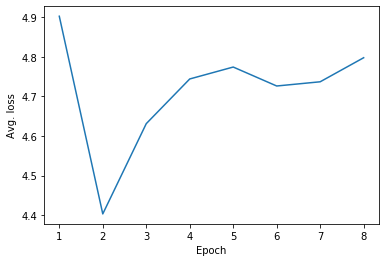
\includegraphics[width=\textwidth]{figures/unsupervised_approach/loss_avgs.png}
    \caption{Avg. training loss of each epoch.}
    \label{fig:loss_avgs}
  \end{subfigure}
  \hfill
  \begin{subfigure}[t]{0.5\textwidth}
    \centering
    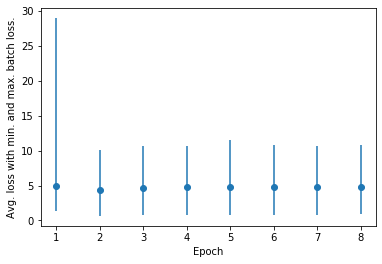
\includegraphics[width=\textwidth]{figures/unsupervised_approach/loss_avgs_range.png}
    \caption{The dots refer to the avg. epoch loss, while the extrema of the line refer to the min. and max. batch loss of that epoch.}
    \label{fig:loss_avgs_range}
  \end{subfigure}
  \caption{Plots of the training loss of the skip-gram model.}
\end{figure}


\subsubsection{Resulting embeddings}

We have computed the cosine distance between certain words to serve as an example. The cosine distance is also the metric we use to compare subjects and documents. The results can be found in table \ref{tab:embeddings_examples}. We have chosen three pairs of words, each of a different field. `polymer'' and ``monomer'' belong to the realm of chemistry; ``machine'' and ``learning'' usually refer to a family of algorithms; ``magnetic'' and ``resonance'' refer to a medical procedure. The chemistry pair is fed to the skip-gram model 96 times during training; the computer science pair, 1357 times and the medicine pair, 961 times.

Given that the cosine distance is symmetric, we only show one half of the table. Also, the distance of a vector to itself is zero. The table shows that the pairs of words of each field are closer to each other than to the other words. The distance between ``polymer'' and ``monomer'' is the largest of the three, which makes sense, as the model receives this pair of words hundreds of times less than the two others. The smallest distance between words that do not belong to the same field is between the words ``magnetic'' and ''polymer''. This distance is 34 \% larger than the distance between ``monomer'' and ``polymer''. Thus, the word vectors accurately differentiate between words that belong to the same field and those that don't.

As a further example of the semantic expressiveness of the embeddings, we can look at the word ``program'', although it belongs to the same field as the computer science pair, it is not as closely related to them. In fact, it appears 27 times as an input to the model with either of the words ``machine'' and ``learning''. However, this is more often as for the pairs of chemistry and medicine, with which it appears as input 26 and 3 times, respectively. The model was able to identify that ``program'' should be closer to the computer science pair, even if it appeared only one time less with the chemistry pair. Its cosine distance to ``machine'' and ``learning'' are 0.77 and 0.72, respectively. On the other hand, its cosine distance to the rest of the words is above 1.

\begin{table}[]
    \centering
    \begin{tabular}{c|c c c c c c}
       $dist(x,y)$ & monomer & polymer & machine & learning & magnetic  \\
       \hline
       resonance & 0.96 & 0.91 & 0.95 & 0.95 & \textbf{0.21} & \\
       magnetic & 0.88 & 0.82 & 0.98 & 0.98 & & \\
       learning & 1.08 & 1.19 & \textbf{0.41} & & & \\
       machine & 1.02 & 0.95 & & & & \\
       polymer & \textbf{0.54} & & & & & \\
    \end{tabular}
    \caption{Cosine distances between the vectors of certain words. The distances of words of the same field are highlighted in bold.}
    \label{tab:embeddings_examples}
\end{table}